% 直角三角形 3-4-5，C 到 AB 的距离 = 12/5
\documentclass[tikz,border=4pt]{standalone}
\usepackage{ctex}
\usepackage{amsmath}
\usetikzlibrary{calc}
\begin{document}
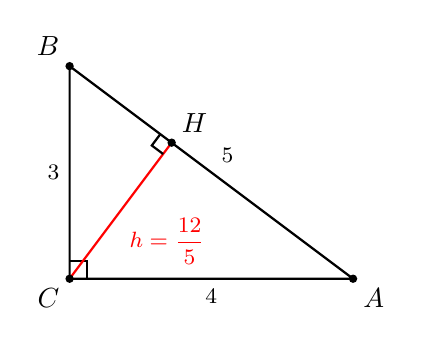
\begin{tikzpicture}[scale=0.9, thick]
  \coordinate (C) at (0,0);
  \coordinate (A) at (4,0);
  \coordinate (B) at (0,3);
  \draw (C) -- (A) -- (B) -- cycle;
  % 直角符号
  \draw (0.25,0) -- (0.25,0.25) -- (0,0.25);
  % 高 CH 到 AB
  % AB 直线：从 A(4,0) 到 B(0,3)，方程 3x+4y=12，单位法向 (3,4)/5
  % C(0,0) 到 AB 距离 = 12/5；垂足 H = 12/25*(3,4) = (36/25, 48/25)
  \coordinate (H) at (1.44, 1.92);
  \draw[red, thick] (C) -- (H);
  % 直角符号 at H：AB 方向 (-4,3)/5，垂线方向 (3,4)/5
  \pgfmathsetmacro{\sz}{0.2}
  \draw ($(H)+(\sz*-4/5, \sz*3/5)$)
     -- ($(H)+(\sz*-4/5 + \sz*-3/5, \sz*3/5 + \sz*-4/5)$)
     -- ($(H)+(\sz*-3/5, \sz*-4/5)$);
  \foreach \pt/\pos in {A/below right, B/above left, C/below left, H/above right}
    \filldraw (\pt) circle (1.2pt) node[\pos] {$\pt$};
  \node[below, font=\footnotesize] at (2,0) {$4$};
  \node[left, font=\footnotesize] at (0,1.5) {$3$};
  \node[above right, font=\footnotesize] at (2,1.5) {$5$};
  \node[red, font=\footnotesize, below right] at (0.7,1.0) {$h=\dfrac{12}{5}$};
\end{tikzpicture}
\end{document}
